% UG project example file, February 2024
%
%   Added the "online" option for equal margins, February 2024 [Hiroshi Shimodaira, Iain Murray]
%   A minor change in citation, September 2023 [Hiroshi Shimodaira]
%
% Do not change the first two lines of code, except you may delete "logo," if causing problems.
% Understand any problems and seek approval before assuming it's ok to remove ugcheck.
\documentclass[logo,bsc,singlespacing,parskip,online]{infthesis}
\usepackage{ugcheck}


% Include any packages you need below, but don't include any that change the page
% layout or style of the dissertation. By including the ugcheck package above,
% you should catch most accidental changes of page layout though.

\usepackage{microtype} % recommended, but you can remove if it causes problems
\usepackage[square,numbers]{natbib} % recommended for citations
\usepackage{graphicx}
\graphicspath{ {./images/}}
\bibliographystyle{unsrtnat}

\begin{document}
\begin{preliminary}

\title{Investigating Machine Learning Techniques for Hearing Aids}

\author{Nikodem Bieniek}

%\course{Artificial Intelligence and Computer Science}
\course{Master of Informatics} % MInf students

\project{MInf Project (Part 1) Report}  % 4th year MInf students
%\project{MInf Project (Part 2) Report}  % 5th year MInf students


\date{\today}

% TOOD: Need to tidy up and expand the abstract
\abstract{
   This dissertation takes the intersection of Machine Learning, Automatic Speech Recognition (ASR) and Hearing Aids (HA) 
   to evaluate the effectiveness of machine learning algorithms in prioritising speech in noisy environments. 
   The aim is to classify the environment based on the audio signal, and then apply heuristic speech enhancement techniques to 
   prioritise speech in particular environments. The experiments are conducted on a novel dataset called HEAR-DS where 
   we evaluate the baseline Convolutional Neural Network (CNN) classifier presented by the authors of the dataset. 
   We then demonstrate techniques that speed up the training process of the CNN model, by using the Adam optimiser. 
   It is also shown that the model can generalise better by applying data augmentation techniques.
   We then compare the performance of the CNN model to a Recurrent Neural Network (RNN) model, specifically 
   the Long Short-Term Memory (LSTM). The results show that the LSTM model outperforms the CNN model. 


   Moreover, we develop a baseline speech enhancement model using a basic CNN model. We then take inspiration 
   from the literatue and apply more layers to the model to improve the performance. We then compare the performance 
   by comparing the STOI and PESQ scores of the models. The results show that the more complex model outperforms the
   baseline model. 
}

\maketitle

\newenvironment{ethics}
   {\begin{frontenv}{Research Ethics Approval}{\LARGE}}
   {\end{frontenv}\newpage}

\begin{ethics}
% \textbf{Instructions:} \emph{Agree with your supervisor which
% statement you need to include. Then delete the statement that you are not using,
% and the instructions in italics.\\
% \textbf{Either complete and include this statement:}}\\ % DELETE THESE INSTRUCTIONS
% %gg
% % IF ETHICS APPROVAL WAS REQUIRED:
% This project obtained approval from the Informatics Research Ethics committee.\\
% Ethics application number: ???\\
% Date when approval was obtained: YYYY-MM-DD\\
% %
% \emph{[If the project required human participants, edit as appropriate, otherwise delete:]}\\ % DELETE THIS LINE
% The participants' information sheet and a consent form are included in the appendix.\\
% %
% % IF ETHICS APPROVAL WAS NOT REQUIRED:
% \textbf{\emph{Or include this statement:}}\\ % DELETE THIS LINE
This project was planned in accordance with the Informatics Research
Ethics policy. It did not involve any aspects that required approval
from the Informatics Research Ethics committee.

\standarddeclaration
\end{ethics}


\begin{acknowledgements}
First and foremost, I would like to solemly thank my supervisor, Hao Tang for 
his enthusiasm in guiding me through this self-proposed dissertation. I am eternally grateful for his wisdom, guidance, and patience throughout the project.

And to my parents, without whose sacrifices I would not have been able to pursue this degree, let alone this project.
\end{acknowledgements}


\tableofcontents
\end{preliminary}


\chapter{Introduction}
\section{Motivations}
Hearing loss is a prevalent condition affecting as much as 
430 million people - or 1 in 18 people. This is expected 
to rise to 1 in 10 by 2050 \cite{WHO2024deafness}.
The most common treatment for hearing loss is the 
provision of hearing technology - such as Hearing Aid (HA) or cochlear implants.
There are many types of HAs, but the most common
type is the behind-the-ear (BTE) hearing aid \cite{Kochkin2010MarkeTrak8}.
However, HA users often report that they struggle to hear speech
in noisy environments. For example, in a study by Kochkin \cite{Kochkin2010MarkeTrak8},
42\% of HA users reported that wind noise was a significant issue for them.
This project aims to evaluate the effectiveness of machine learning algorithms
in prioritising the speech in various environments (such as windy environments).

Modern hearing aids now apply a wide range of techniques to achieve 
better speech prioritisation. For wind noise reduction, this can be achieved 
from mechanical solutions - product design to covers that reduce wind noise - to 
signal processing techniques to compensate for mechanical limitations.
However, current techniques are still not perfect as shown by the study from Kochkin.

Wind noise reduction and indeed, noise reduction in general, is a challenging problem
when paired with speech. This is because you have 
to strike a balance between reducing background noise and
preserving speech. 
Korhen's paper \cite{Korhonen2021WindNoise} outlines 
various techniques that could be used to reduce the wind noise in hearing aids -
from modulation-based noise reduction algorithms (Wiener filtering),
adaptive filtering algorithms, to machine learning techniques.
The paper mentions that the the proposed ML technique:
Long Short-Term Memory (LSTM) neural networks provided
modest improvements in wind noise reduction, however, it did highlight
that ML techniques may still have utility through further research 
and careful algorithmic choices. 

This project aims to pair the proposed machine learning techniques with
signal processing techniques to evaluate the effectiveness of 
speech prioritisation in noisy environments. The idea is to first 
perform acoustic scene analysis (ASA) to classify the environment
based on the audio signal. Afterwards, speech enhancement 
techniques will be applied to the signal to prioritise speech.
ASA can be done using a dataset of varying environments, and 
using machine learning techniques to classify the environment.

In this project, we will be using a novel dataset proposed by \citet{Huwel2020HearDS}
This dataset (called HEAR-DS) is unique because it is specially tailored for HA signal processing and contains
various environments. Normally, voice activity detection (VAD) is used to
detect speech, however, the dataset helpfully contains 
labels which samples contain speech. This can be used 
to implicitly train the machine learning model to classify the environment 
and whether speech is present. Additionally, the paper presents an 
elementary example of how the dataset can be used: to classify the environment -
it showcases the use of a
convolutional neural network (CNN) to classify the environment.
This project will be extending the paper by actually using the dataset 
and comparing various machine learning techniques to evaluate the
effectiveness of the proposed machine learning techniques. 

This project will investigate how recurrent neural networks (RNN) and 
their variants, such as LSTMs, can be used to classify the environment.
 Based on the environment classified, the system will then apply
signal processing techniques to enhance the speech. 
The project 
however has to be mindful in its algorithmic choices - as the computational
power required in HA is limited. It is difficult to pinpoint the exact computational power of a HA
due to the proprietary nature of the devices. In August 2024,
Phonak (Sonova Holding AG) released a new HA which is their first AI 
equipped HA. The device is said to be capable of handling 7,700 Million 
Operations Per Second to accommmodate its neural network with 4.5 million parameters \cite{Hasemann2024PhonakSphere}.  Contrast this with a paper 
from 2021 investigating techniques in VAD for hearing aids 
quotes that it `rarely exceeds 5 million instructions per second (MIPS)` \cite{Gomez2021MIPS}
Moreover, Apple's release of a FDA approved hearing aid in which was previously a mainstream earphone wearable,
Apple Airpods, also shows that there's more interest in this area.
So suffice to say, the computational power of hearing aids is accelerating 
and is most likely going to continue to grow. 

Delay constraints are also
important in HA, as the user needs to hear the speech in real-time.
For example, so long as the speech production is no higher 
than 30 milliseconds (ms), and ideally less than 20ms, the user
is unaffected by the delay \cite{Stone2002Delays}.


% Thus, the evaluation plays a crucial role in this project. From
% objective measures such as the short-time objective intelligibility (STOI)
% and perceptual evaluation of speech quality (PESQ), to quantitative
% measures such as multiply-accumulate operations (MACs) and delay requirements or
% real time factor (RTF) i.e. how fast a system can compute a speech result. 
% The combination of these measures will provide a comprehensive evaluation
% of the proposed machine learning techniques.
%

The project is predominantly aimed at the hearing aid industry. If successful, the project
could advance the state-of-the-art techniques in hearing aids.
Which in turn could improve the quality of life for hearing aid users.
A secondary goal is to make hearing aid research more accessible to the 
computer science community.
The project also hopes to benefit other fields that deal with audio signal processing,
such as mainstream wearables like headphones or microphones.

% \section{Contributions}


\section{Structure}
% The paper is structured as follows:
% \begin{itemize}  
%    \item \textbf{Background} - This chapter will give a high level overview of hearing loss, the auditory system, and the speech processing concepts needed to understand the project.
%    We briefly also cover the two techniques that will be used in this project: Acoustic Scene Analysis (ASA) and Speech Enhancement
%    and some of the related work done in the field. Lastly, I mention the criticism of the paper by \citet{Huwel2020HearDS} 
%    that I will be exploring in this project.
%    \item \textbf{Experimental Setup} - This chapter will cover the datasets that will be used in this project, the baseline models that will be used, and the hypotheses that will be tested.
%    \item We then move onto the results of the experiments.
%    \begin{itemize}
%       \item \textbf{Acoustic Scene Classification} - This section will cover the results of the experiments pertaining to the ASA task.
%       \item \textbf{Speech Enhancement} - This section will cover the results of the experiments pertaining to the speech enhancement task.
%    \end{itemize}
%    \item \textbf{Discussion/Conclusion} - This chapter will discuss the results of the experiments and the implications of the results.
% \end{itemize}
 

\chapter{Background}
% We will begin by briefly giving a high level overview of hearing loss, before discussing 
% what the current treatment and future of hearing loss treatment looks like. We will 
% end on the techniques used to enhance speechV

\section{Hearing Loss}
\subsection{Auditory System}
For sound to be registered by humans, it has to travel through the ear to transform them into
what is known as a neural impulse which is then trasmitted to the brain. We will 
give a high level overview of the process which was collated by the phonetics textbook from \citet{Wayland2018Phonetics},
 but for further reading, refer to the textbook. 
 This process of sound to be registered by humans, is all done in what's known as the Auditory System.
 Figure \ref{fig:ear} shows a birds eye view of the auditory system, and it can be split into three segments
 that we will explore below.

\begin{figure}[h]
   \centering
   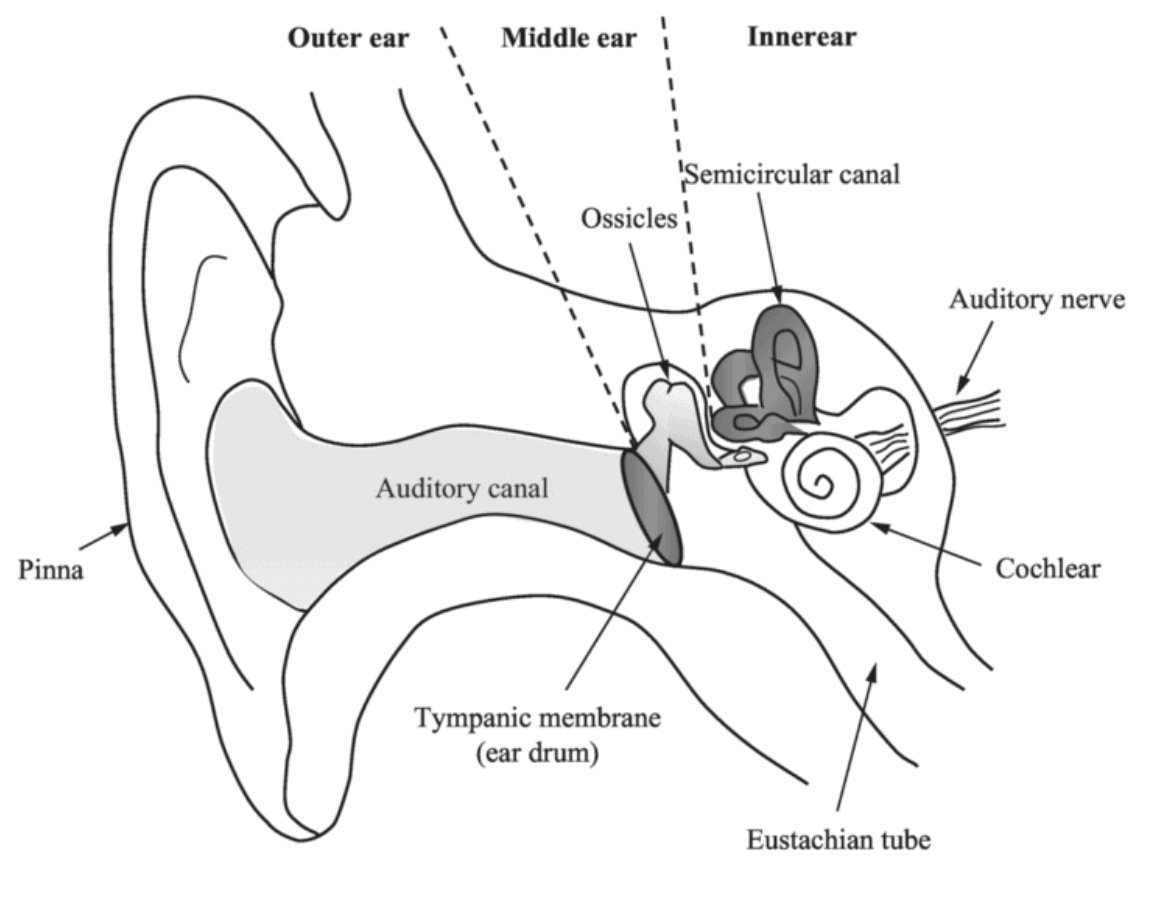
\includegraphics[width=0.5\textwidth]{wayland-ear}
   \caption{The external, middle and the inner ear from \citet{Wayland2018Phonetics}}
   \label{fig:ear}
\end{figure}

\subsubsection{The Outer Ear}
The outer ear (sometimes referred to as the External Ear) is responsible for channeling sound waves to the tympanic membrane (ear drum). Firstly,
sound waves reach the Pinna which funnels it through the auditory canal, and at the end of the canal 
is the ear drum, at which point the sound waves collide with the ear drum which causes the ear drum to vibrate. 
The vibrations are passed along to the middle ear.

\subsubsection{The Middle Ear}
Zooming into the middle ear (Figure \ref{fig:middle-ear}), there are three bony structures: the Malleus, Incus, and Stapes,
and together they make up a lever system. 
It is worth pointing out that when transmitting the energy from the ear drum to the middle ear, there is bound to be some energy 
loss \footnote{Depending on the frequency, this can be as high as 40\%}. The lever system's mechanical advantage 
allows for the sound energy to be amplified so the loss is compensated. 
The Stapes also has an additional function besides passing over the sound vibrations to the inner ear. The Stapes 
is connected by a muscle, the Stapedius muscle, and in response to loud noises, it temporarily increases the stifness
of the bones in the middle ear, which temporarily prevents the acoustic energy to be amplified. This 
protects the inner ear from loud noises.

\begin{figure}[h]
   \centering
   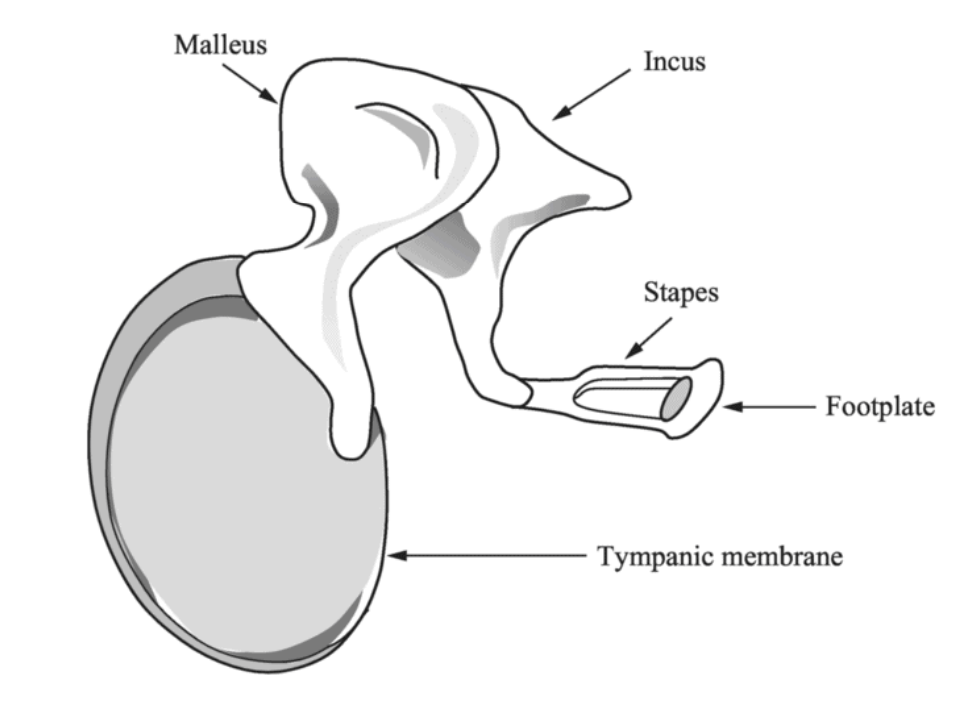
\includegraphics[width=0.5\textwidth]{wayland-middle-ear.png}
   \caption{The components of the middle ear from \citet{Wayland2018Phonetics}}
   \label{fig:middle-ear}
\end{figure}

\subsubsection{The Inner Ear}
One of the parts of the inner ear, is the Cohlea, and it is what gives humans the ability to hear sounds.
The cohlea is a bony structure that resemblers that of a snail shell \footnote{'Cohlea' in Latin translates to snail shell!}.
If the cohlea was unrolled its length would be about 3.5cm, and it is subdivided into various parts (see Figure \ref{fig:cohlear}).
For our purposes, it suffices to know that in the Basilar membrane are a collection of cells, called 
the Organ of Corti, which contain hair cells, and that different hair cells register different frequencies.
Figure \ref{fig:corti} shows the frequency responses shows the various areas of the corti 
and its response to different frequencies. The Organ of Corti is linked to the audtiory nerves and 
so the oscillations that pass through it get coverted to neural impulses and transmitted to the brain.


\begin{figure}[h]
   \centering
   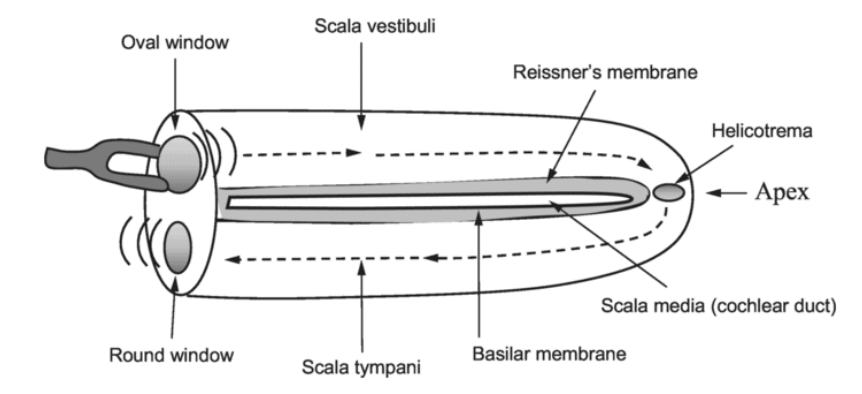
\includegraphics[width=0.5\textwidth]{wayland-cohlear.png}
   \caption{'Unrolled' cohlear from \citet{Wayland2018Phonetics}}
   \label{fig:cohlear}
\end{figure}

\begin{figure}[h]
   \centering
   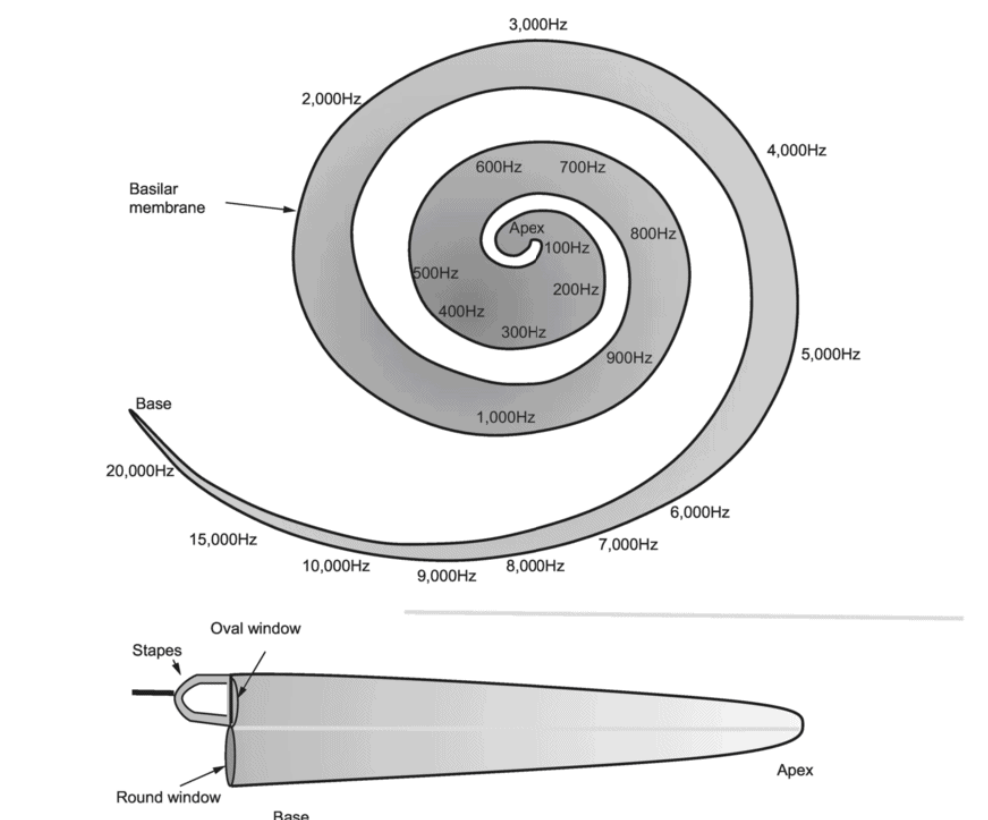
\includegraphics[width=0.5\textwidth]{wayland-corti.png}
   \caption{The Organ of Corti and the frequency responses. From \citet{Wayland2018Phonetics}}
   \label{fig:corti}
\end{figure}

\newpage

% \subsection{Congenital Hearing Loss}
% TODO
% \subsection{Exposure to Loud Noises}
% TODO
% \subsection{Ageing}
% TODO
\subsection{Hair Cell Loss and Hearing Loss}
As we have seen, the hair cells play a major role in allowing humans to register sound. Unfortunately,
it is the major cause of hearing loss since those hair cells are suspectible to damage.
The cause of hair cell loss is complex, since it could be due to many factors such as 
genetic abnormalities (congenital hearing loss), infection, diseases or extrinistic factors such as exposure to loud noises.
It can also occur due to aging, which could be due to the reasons mentioned above, but also 
could be triggered due to age related hearing loss genes. To make matters worse, hair cell loss is unrecoverable in humans \cite{Furness2015HairCell}.
Hearing loss is a spectrum, and varies from mild (26-40dB loss), moderate (41-60dB loss), severe (61-80dB loss) to profound($>80$dB loss) \cite{Nieman2020HearingLoss}.
Moreover, hearing loss may occur in one ear (unilateral) or in both ears (binaural). 

\section{Hearing Loss Treatment}

\subsection{History of Hearing Technology}




\subsection{Hearing Technology}
As mentioned in the Introduction, the most common treatment for hearing loss 
is the provision of hearing technology. There are two common approaches 
to fitting of hearing technology: the equipment of a Hearing Aid (HA) 
or the fitting of a Cohlear Implant. There are similarities in the 
two, and both can be used to fit users that are experiencing profound hearing loss, 
though typically cohlear implants are only considered if the user is experiencing 
a severe hearing loss or further. Another consideration is cost,
the fitting of a hearing aid is a lower barrier of entry since there 
does not need to be any surgical operations done. 

Due to the proprietary nature of the devices, it is unclear what sort of 
algorithms are used in the devices. Though, from Phonak's white paper on Spheric Speech Clarity \cite{Hasemann2024PhonakSphere}
we can deduce that the devices use a combination of ASA and speech enhancement techniques.
From the paper, before signal processing begins, the sound is fed into Autosense OS which 
performs 'scene classification' so in the context of this project, this can be 
considered as an acoustic scene analysis (ASA) algorithm. More specifically, if 
the signal is classified as 'Speech in Loud Noise', then the signal is fed into a 
deep neural network which outputs a mask that seperates the speech signal from the background noise 
which is then applied to the signal. In the context of this project, we will aim to do something similar 
when we train a speech enhancement model on HEAR-DS. 



% It is enough 
% to know for now that the devices will contain multiple microphones, and 
% a dedicated chip which does further processing on the sound depending 
% on the environment the user is faced with.
% It should be pointed out that there is an active area 
% of research into curing congenitial hearing loss - individuals who have been diagnosed with 
% a hearing loss since birth.
% \subsubsection{Hearing Aids}
% Figure ... shows a typical hearing aid, and Figure ... shows the hearing aid labelled.
% TODO
% Microphone info, the reason for multiple mics etc
% There is a surge into rechargable hearing aids.
% Smaller model = higher battery life 

% \subsection{New Approaches to Treatment}
% \subsubsection{Gene-Based Therapy}
% Genitic mutations account for 70-75\% of congenital hearing loss, and with the advent 
% of gene-based therapy, it is not surprising to see that this avenue is explored with hearing loss. 
% However, besides it being an active area of research, it will not be applicable 
% to individuals that have 

\section{Speech Processing Techniques}
\subsection{Digitisation}
To be able to perform speech processing on a device containing a chip/processor (such as a HA), requires us 
to have some sort of digital representation of the sound wave. A waveform is just that, a digital representation 
of the sound we hear. Digital devices can't have infinite precision, so the signal produced by the sound will 
be divided into discrete samples, and the rate at which this occurs is known as the sampling rate. Additionally,
the precision of the amplitude of the signal will be quantized into discrete numbers, and the precision is 
dictated by the bit depth (or the quantization rate).

How do we choose these two values, you may ask? The sampling 
rate will vary between different speech tasks, and part of the decision 
is dictated by a theorem known as the Nyquist-Shannon Sampling Theorem, 
which states that the sampling rate should be at least twice the 
highest frequency range present in the signal. In other words, 
if your speech processing task involves working with frequencies 
of 8KHz, then the sampling rate should be at least 16KHz.
As for the selection of an appropriate bit depth value, 
this depends on the need of representing a wide dynamic range 
of air pressure in a speech signal. Typically, it is 
common to use 16 bits as it can represent an amplitude range of 96dB.

\subsection{Engineered Acoustic Features}
The prevalance of engineering acoustic features in previous work relating to my project and speech processing in general,
warrants a high level overview of this concept to better understand its usage. 
Given some signal $x(t)$, an engineered feature $f(x(t))$ is a function that transforms the signal in some way.
In this project we will be feeding the models the log mel spectrogram of the signal. To obtain the log mel spectrogram, 
we first need to convert the signal (waveform) into the frequency domain (spectrogram).
The process of converting the signal into the frequency domain is done by utilising 
the Fourier Transform. We will technically be using the Fast Fourier Transform (FFT) 
due to efficiency, and the main hyperparameters for the FFT are the window length $w$ 
and the hop length $h$. The window length is the length of the window that is used to 
split the signal into frames, and the hop length is the number of samples between the 
start of each frame. Additionally, there is a choice of a window function and we will 
be using the most common one, the Hann window. Once we apply the FFT, we will be 
left with a complex valued vector of length $w$ and the magnitude of this vector 
gives us the amplitude of the signal at different frequencies. 
We can then apply a Mel Filterbank - a filterbank that is used to mimic the human auditory system. 
Afterwards, we take the logarithm of the filterbank outputs and we are left with the log mel spectrogram.

% In this project we wil be employing the Mel-Frequency Cepstral Coefficients (MFCCs) as our engineered feature.
% The process of extracting MFCSS from waveforms is known as Cepstral Analysis and below are the steps:
% \begin{enumerate}
%    \item Pre-emphasis: Enhances high-frequency components by boosting the signal.
%    \item Windowing: Segments the signal into frames to capture the time-varying nature of speech.
%    \item Fast Fourier Transform (FFT): Converts the signal from the time domain to the frequency domain.
%    \item Mel Filterbank: Applies a filterbank to the FFT output to mimic the human auditory system.
%    \item Logarithm: Converts the filterbank outputs to a logarithmic scale to mimic human perception of hearing.
%    \item Discrete Cosine Transform (DCT): Extracts the cepstral coefficients from the filterbank outputs.
% \end{enumerate}

% \subsection{Acoustic Scene Analysis (ASA)}
% The first step will be 

% \subsection{Blind Source Seperation}

% Blind source seperation 


\section{Related Work}
As this project will chain two algorithms—Acoustic Speech Analysis (ASA) and Speech Prioritization, which is also referred to as Blind Source Separation in some literature—we will cover each in separate sections.
We will discuss the work that has been done and my plans for further development.

\subsection{Acoustic Scene Analysis (ASA)}
Acoustic Scene Analysis is the process of classifying the scene (environment) from an audio stream. For this project 
we will be using a supervised machine learning model for ASA. As such, we need
a sufficiently large dataset that contains useful metadata on the recordings such as the environment it is in.
This project aims to use the HEAR-DS dataset presented by \citet{Huwel2020HearDS}. According to the researchers, 
the dataset came to fruition because existing acoustic scene classification databases are inappropriate for 
HA processing. We will go into more detail of the dataset in Chapter \ref{sec:datasets}.
The paper where the dataset was first introduced, presents the applicability 
of the dataset by showcasing the use of a Convolutional Neural Network (CNN) to classify the environment.
In Chapter \ref{chap:acoustic-scene-classification}, we will be attempting to reproduce the results of the paper. 
As you will see, I struggled to reproduce the results of the paper and I discuss my findings in the chapter too.
So as a validation of the model implementation, I decided to see if the same model parameters 
can be used to classify the DCASE 2017 Acoustic Scenes Challenge dataset \cite{DCASE2017challenge}.
More specifically, I compare \citet{schindler_multi-temporal_2018} model to the CNN model used in the paper.
I discuss my findings in \ref{sec:DCASE-results}.


% But it is enough to know that the dataset is classified in an environment of which it is subcategorised as 
% either containing speech only, background only or speech \& background (both). To prevent machine learning 
% models from overfitting and to increase the diversity of situations, each environment enforces a minimum of three recording situations (REC-SITs) i.e.
% there must be at least three different locations for the recordings. The researchers presented the applicability 
% of this dataset by performing a series of classification experiments using various Convolutional Neural Networks (CNN) of differing sizes.
% This is where the paper could be more clear on the design decisions of the CNN, esepcially because the accuracy of the classification of the models 
% can vary as high as 20\%. This project hopes to reproduce the results, and explain the high variability in the accuracy and how those can be circumvented,
% because the high variability suggests that the random initialisation of weights during training is the primary factor influencing the model performance.
% [To Hao: This is what I understood from your interpretation in the discussion of this paper last Friday, did I understand you correctly?].
% For the recordings labeled as being in environments containing both speech and background noise, the researchers decided against recording the samples in situ.
% Instead they took the speech data from CHiME 
\subsection{Speech Enhancement}

\section{Criticism of Previous Work}
During the course of this project, I found out that the paper by \citet{Huwel2020HearDS} had some issues.
Granted, the paper was more of an exploration of the applicability of the dataset rather than a thorough analysis of the 
performance of the model, it is still important to point out the issues I found. First of all, the paper was not clear 
in the details of the splitting strategy of the dataset so I had to make some assumptions. Additionally, it was not clear 
what loss function was used for training the model. As the dataset only contains raw cuts of the background noise, and 
the researchers opted to mix the speech signal with the background noise so that they have full control over the SNR of the signal,
they used another dataset to mix the speech signal with the background noise. More specifically, they used the CHiMe 3 \cite{barker_third_2015} 
and CHiMe 5 \cite{barker_fifth_2018} datasets. However, only the CHiME 3 development set was used for mixing the speech into the background noise.
CHiME 5 was used for creating a new environment, 'Interferring Speakers', which are samples that contain speech from multiple speakers.
I think using the CHiME 3 dataset and especially only the development set was an odd decision, as there is only roughly 10 hours of data 
from 4 speakers. So a model trained on this dataset may not generalise well to real world scenarios, due to the rich variability of 
speech from different speakers. Nevertheless, we continue with the paper's approach to set up a baseline. Another odd decision was 
in the use of a fixed learning rate scheduler, and the use of a high epoch count without what appears to be no early stopping. This 
will be discussed in more detail in Chapter \ref{chap:acoustic-scene-classification}. We still thank the authors for their work on the dataset 
as it is a promising dataset for the future of HA research.

\chapter{Experimental Setup}
\section{Datasets}
\label{sec:datasets}
\subsection{HEAR-DS}
TODO
\subsection{CHiME3}
TODO
\subsection{CHiME6}
TODO

\section{Baseline Models}

\section{Hypotheses}

\begin{enumerate}
   \item \textbf{Using Fixed Learning Rate Stochastic Gradient Descent (SGD) will result in a longer training time than using Adam Optimiser.} The paper by \citet{Huwel2020HearDS} used the fixed learning rate SGD approach.
   I hypothesise that using Adam Optimiser will result in a shorter training time.
   \item \textbf{Data Augmentation will result in a higher accuracy of the model.} It is unclear from the paper whether the authors used data augmentation...
   \item \textbf{Using an LSTM model will result in a higher accuracy of the model.}
\end{enumerate}


\chapter{Acoustic Scene Classification Experiments}
\label{chap:acoustic-scene-classification}
\section{Data Preparation}
TODO
\subsection{Fixed Learning Rate SGD Approach}
TODO
\subsection{Adam Optimiser Approach}
TODO
\subsection{LSTM Model}
TODO

\chapter{Speech Enhancement Experiments}
\section{Data Preparation}
TODO
\subsection{CNN Model}
TODO

\chapter{Conclusions}
\section{Discussion}
TODO
\section{Future Work}
TODO









% \chapter{Conclusions}

% \section{Final Reminder}

% The body of your dissertation, before the references and any appendices,
% \emph{must} finish by page~40. The introduction, after preliminary material,
% should have started on page~1.

% You may not change the dissertation format (e.g., reduce the font size, change
% the margins, or reduce the line spacing from the default single spacing). Be
% careful if you copy-paste packages into your document preamble from elsewhere.
% Some \LaTeX{} packages, such as \texttt{fullpage} or \texttt{savetrees}, change
% the margins of your document. Do not include them!

% Over-length or incorrectly-formatted dissertations will not be accepted and you
% would have to modify your dissertation and resubmit. You cannot assume we will
% check your submission before the final deadline and if it requires resubmission
% after the deadline to conform to the page and style requirements you will be
% subject to the usual late penalties based on your final submission time.

\bibliography{mybibfile}


% You may delete everything from \appendix up to \end{document} if you don't need it.
% \appendix

% \chapter{First appendix}

% \section{First section}

% Any appendices, including any required ethics information, should be included
% after the references.

% Markers do not have to consider appendices. Make sure that your contributions
% are made clear in the main body of the dissertation (within the page limit).

% \chapter{Participants' information sheet}

% If you had human participants, include key information that they were given in
% an appendix, and point to it from the ethics declaration.

% \chapter{Participants' consent form}

% If you had human participants, include information about how consent was
% gathered in an appendix, and point to it from the ethics declaration.
% This information is often a copy of a consent form.


\end{document}
